\section{Auswertung}
\label{sec:auswertung}

\subsection{Rohdaten}
Die Messwerte tabelliert, inkl. Unsicherheiten:
\begin{table}[H]
  \centering
  \caption{Beispiel-Messreihe mit Unsicherheiten.}
  \label{tab:messreihe}
  \begin{tabular}{S[table-format=2.1] S[table-format=2.1] @{${}\pm{}$} S[table-format=1.1]}
    \toprule
    {t in \si{\second}} & {s in \si{\milli\meter}} & {$\Delta s$ in \si{\milli\meter}} \\
    \midrule
    1.0 & 2.1 & 0.2 \\
    2.0 & 4.3 & 0.2 \\
    3.0 & 6.2 & 0.3 \\
    4.0 & 8.5 & 0.3 \\
    \bottomrule
  \end{tabular}
\end{table}

\subsection{Darstellung}
Aus den Messwerten entsteht eine Ausgleichsgerade. Exemplarisch mit pgfplots:
\begin{figure}[H]
  \centering
  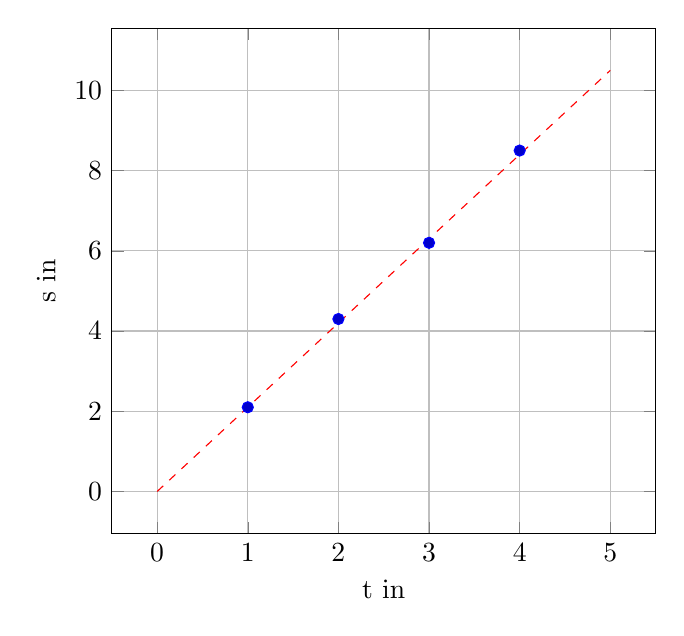
\begin{tikzpicture}
    \begin{axis}[
      width=0.7\textwidth,
      height=8cm,
      xlabel={t in \si{\second}},
      ylabel={s in \si{\milli\meter}},
      grid=major,
    ]
      \addplot+[only marks] coordinates {
        (1.0, 2.1) (2.0, 4.3) (3.0, 6.2) (4.0, 8.5)
      };
      \addplot+[domain=0:5, dashed, no marks] {2.1*x};
    \end{axis}
  \end{tikzpicture}
  \caption{Messwerte mit linearer Ausgleichsgerade.}
  \label{fig:fit}
\end{figure}

\subsection{Fehlerbetrachtung}
Hier werden die Unsicherheiten der Messwerte, der Ausgleichung und der
Ergebnisse aus \cref{eq:gausserror} diskutiert. Beispiel für die Ergebnisnotation:
\begin{equation}
  \errval{12.3}{0.4}\, \si{\milli\meter\per\second}
  \label{eq:ergebnis}
\end{equation}
